\section{Análisis del Péndulo No Lineal}

La dinámica de un péndulo simple con parámetros normalizados ($g/L = 1$) se describe mediante la ecuación diferencial:

\begin{equation}
    \frac{d^2\theta}{dt^2} + \sin\theta = 0
\end{equation}

Al estudiar oscilaciones con amplitudes superiores a los $10^\circ$, el sistema se aleja del régimen armónico simple. La fuerza restauradora no lineal ($\sin\theta$) provoca la pérdida del isocronismo, haciendo que el periodo de oscilación $T$ dependa de la energía inicial. Este fenómeno genera una deriva de fase si se analiza el sistema bajo la premisa de un periodo constante $2\pi$, lo que se evidencia claramente mediante el uso de secciones de Poincaré.

\subsection{Metodología de Muestreo y Periodo Óptimo}

El análisis se fundamenta en un muestreo estroboscópico del espacio de fases $(\theta, \omega)$. Esta técnica reduce la trayectoria continua a un conjunto discreto de estados capturados cada intervalo de tiempo $T_s$. La interpretación de la sección de Poincaré resultante permite diagnosticar la relación entre la frecuencia de muestreo y la dinámica natural del oscilador:

\begin{itemize}
    \item \textbf{Deriva de Fase ($T_s = 2\pi$):} Dado que para grandes ángulos el periodo real es superior a $2\pi$, el péndulo se encuentra en una fase distinta en cada instante de captura. La sección de Poincaré muestra una sucesión de puntos que delinean gradualmente la órbita, revelando la deformación geométrica de la trayectoria en comparación con la elipse característica del régimen lineal.
    \item \textbf{Punto Fijo y Periodo Óptimo ($T_s = T_{real}$):} El periodo óptimo es aquel que coincide exactamente con el tiempo de retorno del sistema para una amplitud dada. En esta condición, la sección de Poincaré colapsa en un único punto estable $(\theta_0, 0)$, confirmando la sincronización entre el intervalo de captura y la periodicidad intrínseca del sistema.
\end{itemize}

\subsection{Implementación Numérica y Determinación del Periodo}

Para la integración temporal, el sistema se descompone en un par de ecuaciones de primer orden: $\dot{\theta} = \omega$ y $\dot{\omega} = -\sin\theta$. Se emplea el algoritmo de Runge-Kutta de cuarto orden (RK4) para asegurar que la trayectoria permanezca sobre la curva de energía constante sin degradación por errores de fase acumulados.

Debido a que el periodo no es constante, se implementa una técnica de detección de picos basada en el monitoreo de la velocidad angular. Partiendo del reposo con una amplitud $\theta_0$, el periodo natural $T_{real}$ se estima identificando el instante en que la velocidad completa un ciclo de oscilación:

\begin{equation}
    \omega(t_{i-1}) > 0 \quad \text{y} \quad \omega(t_i) \leq 0 \implies T_{real} \approx t_i
\end{equation}

Este procedimiento permite obtener el valor preciso para el muestreo estroboscópico. Complementariamente, se realiza un bosquejo del espacio de fases global para visualizar la topología de las órbitas cerradas. A amplitudes elevadas, la deformación de las elipses hacia formas ovoides ilustra cómo el sistema permanece más tiempo en las zonas de máxima elongación, justificando físicamente el incremento del periodo respecto al caso lineal.

\subsection{Código Fuente}

La simulación se centra en la integración del sistema mediante el algoritmo Runge-Kutta de cuarto orden (RK4), aplicado a una amplitud inicial de $60^\circ$ para asegurar un régimen no lineal evidente. La estructura computacional se divide en tres procesos clave: la definición de la dinámica sistémica, un algoritmo de detección de eventos para el cálculo del periodo natural y un motor de muestreo estroboscópico para la construcción de las secciones de Poincaré.

Para la determinación del periodo óptimo ($T_{real}$), se emplea un monitor de estados que identifica el instante exacto en que la velocidad angular $\omega$ cruza por cero con pendiente negativa, indicando que el sistema ha completado una oscilación y regresado a su elongación máxima. Este valor se utiliza posteriormente como intervalo de tiempo para el muestreo de Poincaré, permitiendo comparar la respuesta del sistema frente al periodo lineal teórico ($2\pi$).

El código fuente detallado se encuentra en el archivo adjunto y se integra a continuación:

\lstinputlisting[
    language=Python,
    caption={Simulación del Péndulo No Lineal y Secciones de Poincaré},
    label={code:pendulo}
]{src/exercise03.py}

En la implementación, se incluye además un bosquejo del espacio de fases global. Este procedimiento permite visualizar la topología de las órbitas cerradas para distintas energías, evidenciando cómo la geometría de la trayectoria se aleja de la circularidad ideal del oscilador armónico a medida que aumenta la amplitud inicial. Este mapeo integral es fundamental para contextualizar la posición de los puntos obtenidos en las secciones de Poincaré.

\subsection{Análisis de Resultados y Discusión Técnica}

\begin{figure}[H]
  \centering
  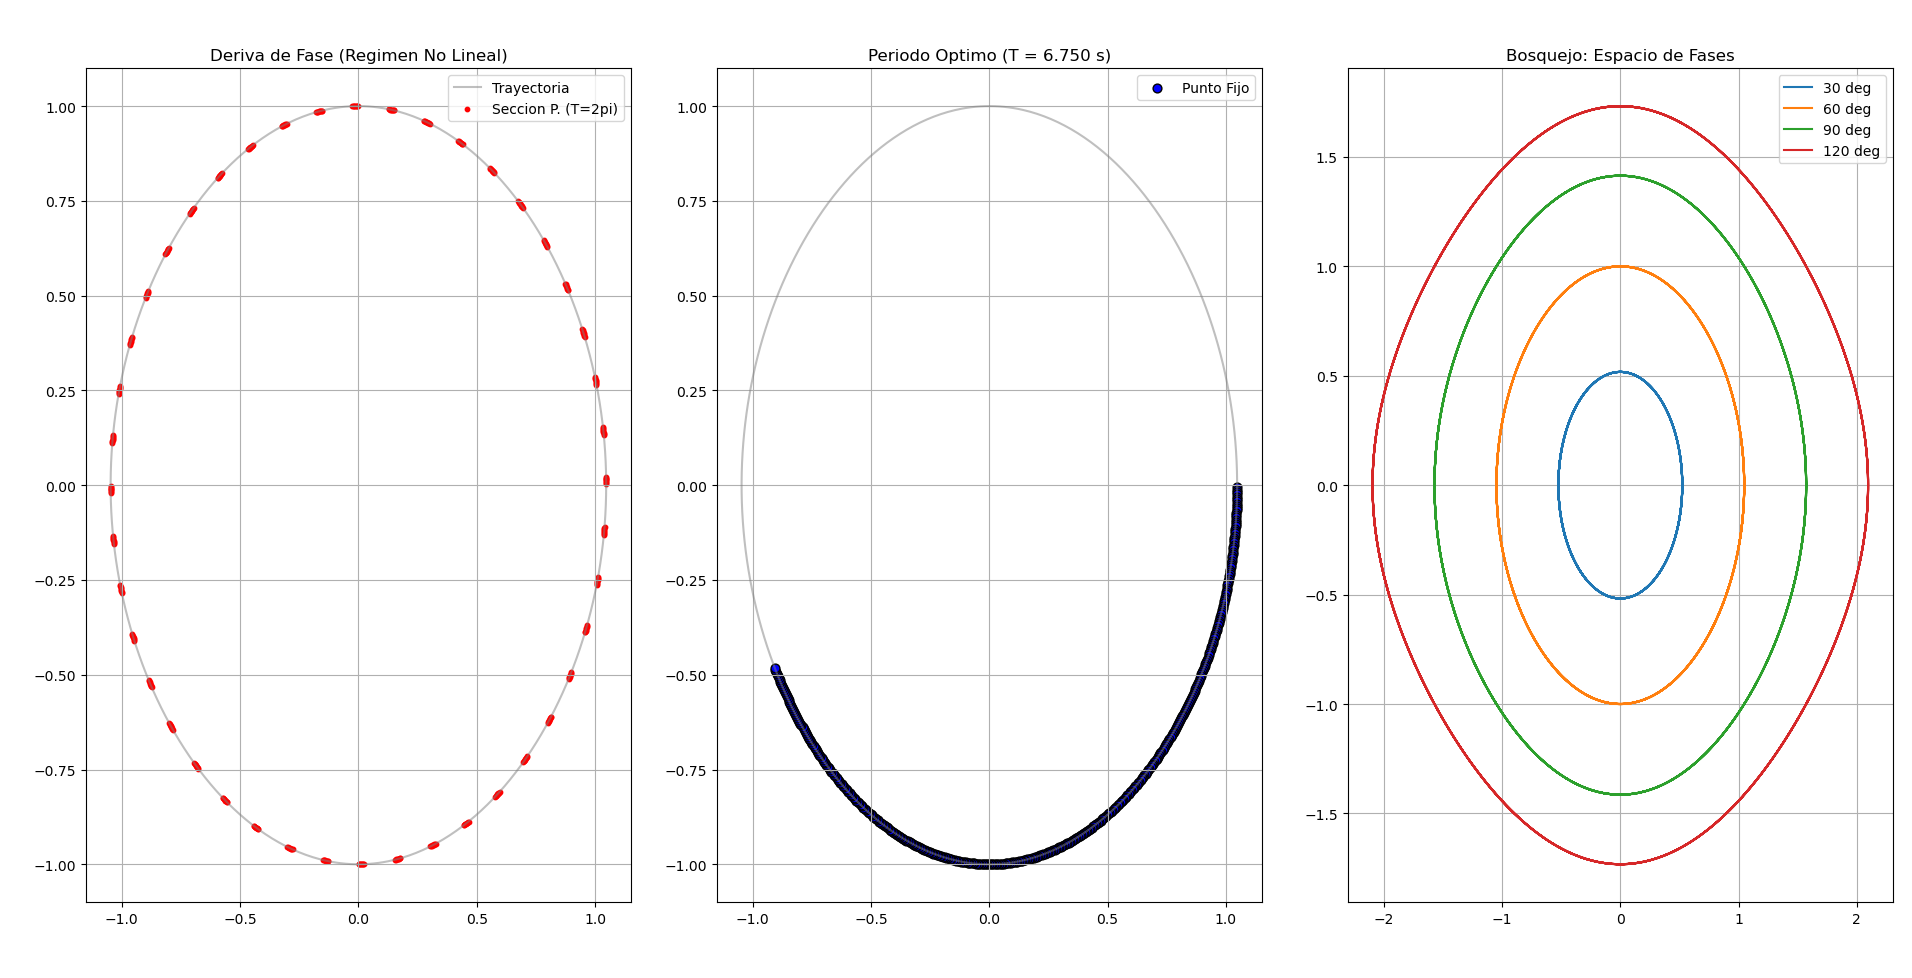
\includegraphics[width=0.9\textwidth]{img/report/exercise03.png}
  \caption{Solución computacional}
  \label{fig:exer03}
\end{figure}

Tras la ejecución del modelo computacional para una amplitud inicial de $\theta_0 = 60^\circ$ ($1.047$ rad), se obtuvieron los resultados visualizados en la figura analizada. El análisis se desglosa en los siguientes ejes fundamentales:

\subsubsection{Cuantificación del Periodo y Desviación No Lineal}

El primer resultado relevante es la obtención del periodo natural mediante el algoritmo de detección de picos. Para la condición inicial de $60^\circ$, el sistema reporta un periodo óptimo de $T_{real} = 6.750$ s. Al comparar este valor con el periodo teórico del régimen lineal ($T_0 = 2\pi \approx 6.283$ s), se observa un incremento del $7.43\%$. 

Esta diferencia métrica es el fundamento del comportamiento observado en las secciones de Poincaré. Mientras que en un oscilador armónico el periodo es independiente de la amplitud (isocronismo), aquí la no linealidad del potencial gravitatorio ($V(\theta) = 1 - \cos\theta$) ralentiza el movimiento a medida que la elongación aumenta, un fenómeno capturado con precisión por el integrador RK4.

\subsubsection{Interpretación de las Secciones de Poincaré}

El análisis estroboscópico revela la naturaleza del mapeo de fase del sistema:

\begin{itemize}
    \item \textbf{Análisis de la Deriva (Panel Izquierdo):} En la sección de Poincaré con $T = 2\pi$, los puntos rojos no colapsan, sino que se distribuyen a lo largo de toda la trayectoria. Esto ocurre porque el intervalo de muestreo es más corto que el ciclo físico del péndulo. En cada "foto" estroboscópica, el sistema se encuentra en un estado de fase retrasado respecto al anterior, lo que visualmente genera una reconstrucción de la órbita completa. Este resultado es una prueba computacional de la asincronía inducida por la no linealidad.
    \item \textbf{Validación del Punto Fijo (Panel Central):} Al ajustar el muestreo al periodo óptimo calculado ($6.750$ s), los puntos azules tienden a concentrarse en una región específica del espacio de fases ($1.047, 0.0$). La reducción de la sección de una curva a un cúmulo localizado confirma que se ha identificado la periodicidad fundamental del sistema. La pequeña dispersión o "arco" observable en este panel es un indicador de la sensibilidad numérica: incluso una discrepancia mínima entre el paso de integración $h$ y el periodo real acumulado durante cientos de ciclos genera una deriva detectable, lo que subraya la importancia de la precisión del método RK4 empleado.
\end{itemize}

\subsubsection{Topología del Espacio de Fases (Bosquejo)}

El panel derecho presenta el "bosquejo" del espacio de fases para múltiples condiciones iniciales ($30^\circ$ a $120^\circ$). Computacionalmente, este gráfico permite observar la transición geométrica de las órbitas:
\begin{enumerate}
    \item A bajas amplitudes ($30^\circ$), la órbita es sensiblemente elíptica, aproximándose al comportamiento de un círculo en unidades normalizadas.
    \item A amplitudes elevadas ($120^\circ$), la trayectoria se deforma hacia una geometría ovoide más achatada. Físicamente, esto indica que el péndulo permanece proporcionalmente más tiempo en las regiones de alta energía potencial (extremos de la oscilación) comparado con un oscilador lineal, lo que explica el aumento del periodo observado anteriormente.
\end{enumerate}

\subsection{Conclusiones de la Simulación}

El estudio realizado permite concluir que la sección de Poincaré es una herramienta diagnóstica excepcional para sistemas no lineales. Se ha demostrado que el periodo óptimo es el único parámetro que permite la reducción dimensional de una órbita a un punto fijo en el mapeo estroboscópico. Asimismo, la concordancia entre el bosquejo del espacio de fases y las derivas observadas en el muestreo lineal valida el modelo de péndulo simple no lineal y la eficacia del algoritmo RK4 para conservar la estructura simpléctica del sistema durante tiempos de simulación prolongados.
